%%This is a very basic article template.
%%There is just one section and two subsections.
\documentclass[a4paper]{article}
\usepackage{amssymb}
\usepackage{amsmath}
\usepackage{graphicx}
\usepackage{subfigure}
\usepackage{soul}
\usepackage{color}

% soul highlighting config
\setul{1ex}{0.8ex}
\definecolor{orange}{rgb}{1,0.5,0}
\setulcolor{orange}


\begin{document}
	\begin{titlepage}
	
	\centering
	
	{\huge\bfseries Management Dashboard with IBM Cognos\par}
	\vspace{2cm}
	
	
	\begin{figure}
    \subfigure{
\includegraphics[width=0.25\textwidth]{FH}\par\vspace{1cm}}
    \hspace{5cm}
    \subfigure{
\includegraphics[width=0.25\textwidth]{KABEG}\par\vspace{1cm}}
	\end{figure}
	\vspace{1.5cm}
	
	{\Large\itshape Christopher Schmidt\\
	Fabian Matschitsch\par}
	\vfill
	supervised by\par
	Dr.~Florian Hollomey\\
	Dipl. Ing. Gerhard Orlitsch
	\vfill
	{\large \today\par}	
	
	\end{titlepage}

	\tableofcontents
	\newpage

	\section{Introduction}
	The Board of Directors of the Klinikum Klagenfurt is required to get
	key data from the Hospital Information System for
	meetings and presentations independent from the IT department.
	They commissioned us to implement a Management Dashboard for statistical
	data out of the Hospital Information System (HIS) and the ELGA System. The Management Dashboard
	should be based on Cognos Database Cubes from the HIS and the ELGA Databases.\\
	\\
	It should be possible to display key figures on the IBM Cognos
	Webportal and the Mobile App obtained from diagrams, charts and tables.
	In addition, it should be possible to get statistical data with a
	simple click on a link in a browser or with the IBM Cognos Mobile Application.\\
	\\
	To get such charts, tables, etc., users specify their parameters like
	departments, stations, wards, in-patient or out-patient-flag within
	pre-designed forms. A simple button click delivers the specified key values in
	the requested format.\\
	The major advantage is that the directors have no direct linkage to the
	IT Department and that they can get their results (for example, a comparison of
	key-values over years) with a few clicks in the Website or the Mobile
	Application on their own.
	\newpage
	
	\section{Hospital Information Communication}
		The communication in hospitals is mainly about patient data,
		medical and laboratory results, radiographs, financial data, insurance
		data and the like. This chapter describes the communication in gernal.
	\subsection{General Communication}
		The Hospital Information System (HIS) provides a major
		platform for this kind of communication. HIS stores patient information and
		sends data to other subsystems. A subsystem can be every system which needs
		patient-related data. A subsystem can send data back to HIS, too.
		For the communication  process between the systems, a standardized
		protocol, named Health Level 7 (HL7), is used. The following list gives
		examples for subsystems of the Hospital Information System:
		\begin{itemize}
	    	\item Laboratory Information System (LIS)
	    	\item Electronic Medical Record (EMR)
	    	\item Pharmacy Management (PM)
	    	\item Insurance Management (IM)
	    	\item Financial System (FS)
	    	\item Radiology Information System (RIS)
	    	\item Appointment Management (AM)
	    	\item Emergency Management System (EMS)
	    \end{itemize}
	    \begin{figure}[!ht]
		  \centering
		      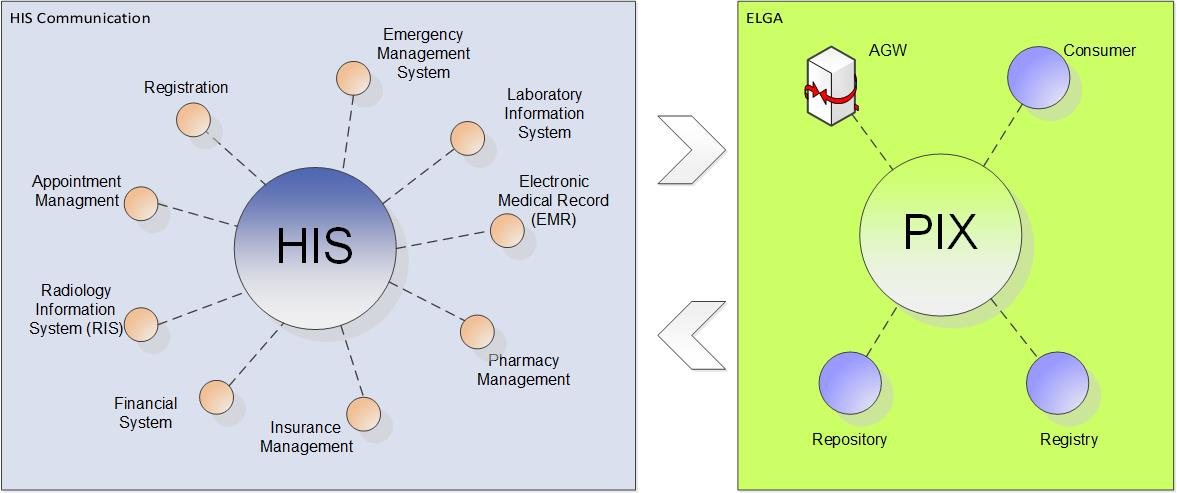
\includegraphics[width=1.0\textwidth]{HIS_Overview}
		  \caption{The blue box on the left illustrates the communication of the
		  Hospital Information System. HIS  communicates with the ELGA system
		  (on the right) which has its own Patient Identifier Cross Referencing
		  (PIX) and a Access-Gateway (AGW) for connecting and communicating with
		  external partners.}
		\end{figure}
	    A Special system for patient-related documents is called for Austria,
	    where citizens can restrict the access of others to their data. The system
	    is called Elektronische Gesundheitsakte (ELGA).
	    This gives people in Austria the possibility to have a look at their
	    own clinical records on a digital basis. ELGA and its architecture will be
	    explained in chapter 4.\\
	    The systems speak to each other via a communication server.
	    This communication server connects all systems, maps different
	    types of messages in other structured layouts so that they can be
	    understood by other systems and can retrieve and store messages.
	\subsection{Health Level 7}
		The Health Level 7 (HL7) is a standardized protocol in version 2.5. In
		the near future, version 3 will be used for the communication  process in
		eHealth systems.
		All systems communicating in hospitals are called eHealth
		systems.\\
		HL7 provides a framework to exchange, integrate, share and retrieve 
		electronic health information. It defines the language, the structure and the
		data types which are used for the communication process between the eHealth
		systems.\\
		The standard is human-readable and nearly all eHealth systems are able to
		read data from HL7 and export data to HL7.
		
	\newpage
	
	\section{IBM Cognos Business Intelligence}
	IBM Cognos Business Intelligence (BI) is a software suit designed to extract
	corporate data from data sources. A data source is everything from which
	persistent information can be retrieved. The extracted data can be assembled in
	the Framework Manager environment to build a so called data warehouse. This
	warehouse forms a foundation from which reports can be created and executed in
	Report Studio. After reports are created, users can run HTML-based reports in
	Cognos Webview. Features like automated processes, user policies, restricted
	access to reports, etc, are supported.
	
	\subsection{Framework Manager}
	The Framework Manager allows the construction of a logic layer, uniting different data sources in terms of 'query
	items', which grant the possibility of defining customized queries over, for
	example, multiple tables in one single logical item. Also the filtering of
	retrieved data can be done.
	\subsubsection{Defining Data Sources}
	Before data can be gathered in the Framework Manager, database connections have
	to be established for the Cognos application. Because Cognos can run on a
	Windows server, drivers have to be installed for each type of database. This
	can be done in 'ODBC Data Source Administrator'-Tool. When arranging a
	connection for the first time, the appropriate data source type for the
	connection has to be chosen. This could be ODBC, ANSI or a mixed type for 32-
	and 64 bit data sources. The figure below gives a sample:\\
	\begin{figure}[!ht]
		  \centering
		      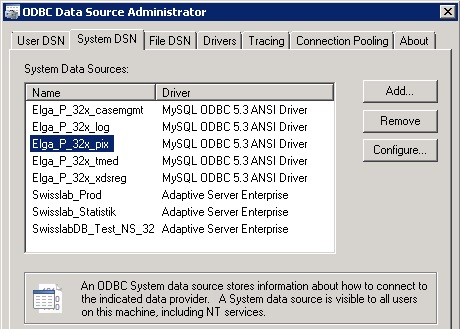
\includegraphics[width=0.6\textwidth]{ExistingDataSource}
		  \caption{Example for Datasources in the Framework Manager}
	\end{figure}\\
	Furthermore, connection details for the database have to be entered for every
	connection.
	\subsubsection{Frame Manager Surface}
	Because patient-related information is used, it must be evaluated what may
	revealed. The following figure gives an example for an existing
	data warehouse:
	\begin{figure}[!ht]
		  \centering
		      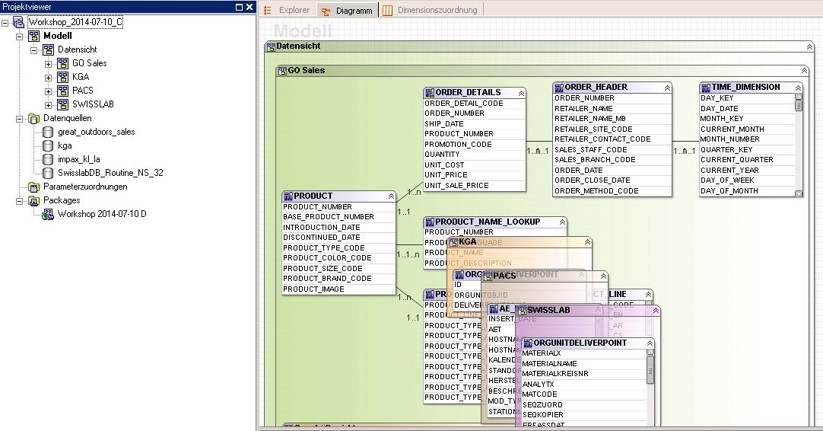
\includegraphics[width=0.8\textwidth]{frameworkM_2}
		  \caption{Example for an existing data warehouse}
	\end{figure}
	On the left side the project viewer can be seen. It displays in general logical
	items. These can be data sources, views of data sources, which can be modified
	without altering existing data, and query items. Query items itself are highly configurable and allows to define customized and complex
	queries, which would not be possible by selecting data directly.\\
	\\
	In a centered position, the data view can be seen. It is a graphical surface
	allowing the creation of logic relations between tables or query items.
	Filtering of selected data can also be done in this view. With filters
	simply all the data can be selected in terms of performance and shrinked
	afterwards. This greatly increases performance without stressing data sources.
	Beside the usage of logical relations and filters, the creation of
	dimensions is possible.
	This can be done in 'Dimensions', which can be seen at the top of the figure. 
	Dimensions allow the comparison of
	key figure dependencies on dimensions like time, costs, storage usage and
	more.\\
	\\
	When the construction of a data warehouse is done, or changes on data are
	performed, a package must be published in order to create reports in the Report
	Studio.
	\subsection{Report Studio}
	Report Studio allows the creation of HTML-based reports for end users
	(Business users in Cognos terms), which can be executed on demand or
	time-based.
	\begin{figure}[!ht]
		  \centering
		      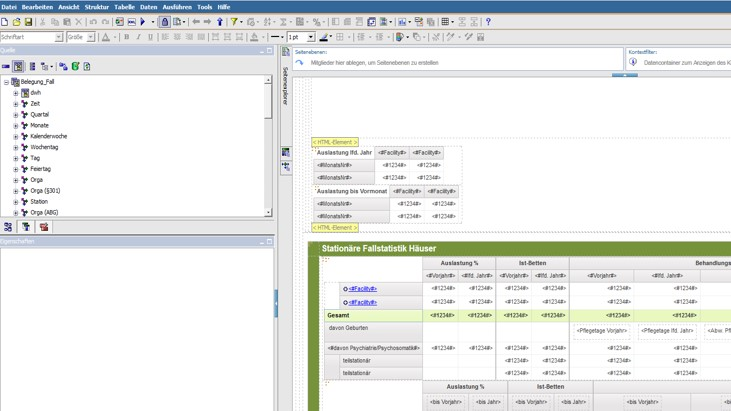
\includegraphics[width=0.6\textwidth]{ReportStudio_2}
		  \caption{The figure shows the graphical output of Report Studio.}
	\end{figure}
	On the left side query items, dimensions and simple numbers can be seen, which
	were created with the Framework Manager. In the centered view the general
	structure of the report can be assembled by simply drag-and-drop
	elements wanted in the view. Also text, graphical elements and different types
	of diagrams can be added
	\subsection{Data Topology of Cognos}
	As mentioned, Cognos forms a logical data level consisting of
	physical data sources. In Frame Work Manager, query items, dimensions, numbers
	and more can be defined. After the data ware house has been assembled, reports
	can be built in Report Studio and provided to Business Users. This can be seen
	in the following figure:
	\begin{figure}[!ht]
		  \centering
		      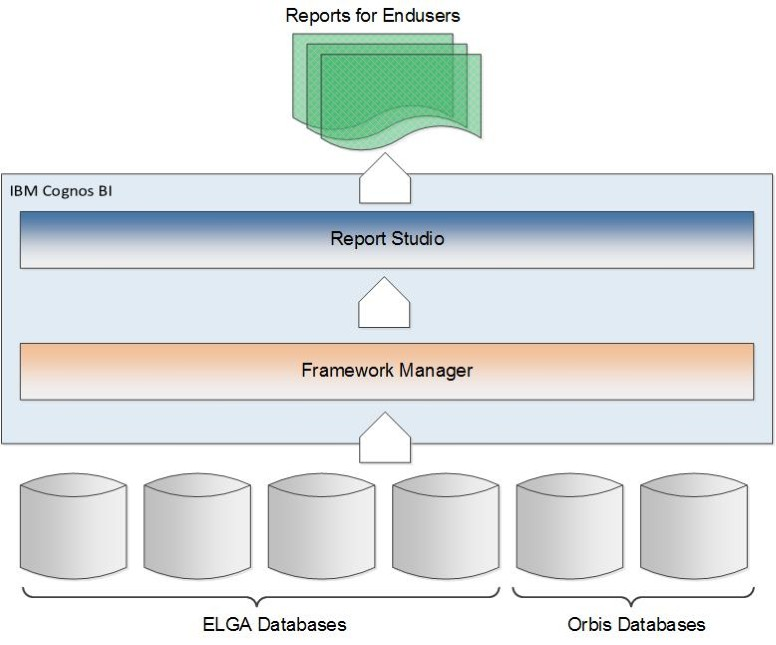
\includegraphics[width=1.0\textwidth]{AllDBtoCognos}
		  \caption{Figure shows how the databases will be connected to Cognos.}
	\end{figure}
	
	\newpage
		
	\section{ELGA }
	In the second quarter of year 2016, ELGA in Carinthia (now on referred as 'ELGA
	Bereich Kaernten' (EBK)) will be connected to central core components. This connection
	will make the availability of documents of citizens and 
	non-citizens possible in Austria. Today, the EBK operates
	as an isolated unit which receives data solely from Carinthian healthcare
	providers.
	At the moment there is no knowledge about quality, correctness and the total
	amount of data. This knowledge is urgently needed in decision-making processes.\\
	\\
 	This lack of knowledge should be compensated by the use of IBM Cognos Business 
 	Intelligence, a multi-database environment, by creating a data-warehouse in the KABEG-IT
 	department. A data-warehouse forms a model in a central place consisting of
 	several sources of persistent information.\\
 	\\
	The aim of this project is to build up a prototype model for the ELGA environment from 
	scratch, using the existing databases. On the basis of this model, HTML-based reports 
	for end-users should be created, which should give the current amount of
	patients, registered documents (local and remote ones), queried documents,
	the number of accesses of users and performance of transactions. When the EBK
	goes live, a distinction between regional-ELGA-relevant documents, also called 'Informationsverbund-documents' (IV)
	and EBK-documents will be accomplished. This distinction will be integrated
	into the reports.\\
	\\
	
	\subsection{XDS - Cross Document Sharing}
	
	The concept of ELGA, in this case IV and EBK, is described by the term Cross Document Sharing
	(XDS), which allows the exchange of documents between health care providers,
	also on federal state level.\\
	This requires the following components:\\
	\begin{itemize}
	    	\item PIX - Patient Identifier Cross-Referencing\\
	    	Each ELGA realm uses its own PIX for managing patients. A central patient index is used to
	    	make cross document sharing possible.
	    	\item Registry\\
	    	In general the main task of the registry is to link patients with their
	    	related information and also documents.
	    	In detail, the jobs and functions of a registry are much more complex.
	    	\item Policy Repository\\
	    	Access to documents is managed  by a policy repository. The compliance of patients is entered
	    	by care personnel, which can also be administrative personnel for example.
	    	For EBK-related employees this process is similar, but instead of using
	    	the local repository a central authorization system is used. This allows citizens to manage access to their documents any time.
	    	\item XDS Repository\\
	    	A repository which consists of multiple logical storages. It saves and provides documents
	    	for health care providers.
	    	\item XDS Consumer\\
	    	A consumer has the role of a client. It retrieves documents from the XDS
	    	repository for users.
	    	\item AGW - Access Gateway\\
	    	The main task of the AGW is to connect the EBK to central components and
	    	make Cross Community Access (XCA) between ELGA realms possible.
	    	\item ATNA - Audit Trail and Node Authentication\\
	    	Every transaction from any node is protocolled in an ATNA repository.
	    	This forms the largest source upon which the reports are built.
	    	
	 \end{itemize}
	
	
	
	\subsection{Data Model}
	The basic structure of the ELGA data model consists of an Electronic Business
	XML - database (ebXML).
	Will be written when ELGA goes online, because major
	changes to the model will be made.
	Because ELGA handles patient-related data, it must be evaluated how far the
	model can be described.
	\subsection{Evaluation and Measurement of Key-Figures}
	Will be written when ELGA goes online, because major changes to the model
	will be made. Because ELGA handles patient-related data, it must be evaluated
	how far the key-figures can be described.
	\subsection{Next Steps}
	The next project steps are the finalization of the prototype model and the
	extension of reports. The finalization focuses on the investigation of
	different data warehouse schemes in aspects of time-efficiency and stress-minimization of the running system.
	The reports will be supplemented with a fraud detection-report, which is supposed to 
	show information about unpermitted and irregulary access of users.
	Furthermore, several fraud detection techniques will be investigated. As EBK goes online, a major
	update of software and datamodels will be implemented, making adaption and
	changes of the existing data-warehouse necessary. On the other hand, this could
	lead to new possibilities and additional information in the data-warehouse.
	
	\newpage
	
	\section{Hospital Information System - AGFA Orbis}
	The Hospital Information System forms the central plattform in
	the inter-clinical communication. All the patient data will be stored in this
	system, and all the booking and timebased terms for patients will be made
	there.\\
	In the KABEG there are five hospitals and two Hospital Information
	Systems. In the future, a major change will be made so that only one
	HIS is in use within KABEG. This will be solely AGFA Orbis.
	\subsection{Orbis in the KABEG}
	At the moment, only four of five KABEG hospitals are using AGFA Orbis as HIS.
	The main functionality of Orbis is to collect all patient data and to
	distribute data to subsystems. Beside its main task, Orbis has much more
	functionalities.\\
	Orbis consists of modules which are connected to one system. One
	of these modules is the appointment calendar. The users can plan
	patient appointments and additional events, but the calendar can also be used
	for internal schedules and notes.
	Another module is the planning and documentation of surgeries. In this module
	users have a view of all the operating rooms and can see when patients
	come, when a surgery starts and ends and much more.\\
	\begin{figure}[!ht]
		  \centering
		      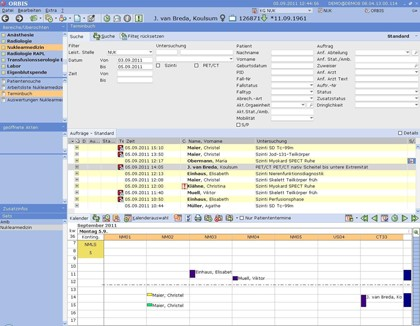
\includegraphics[width=0.6\textwidth]{orbis1}
		  \caption{Orbis Appointment calendar. User can plan 
		  patients appointments and their own terms.}
	\end{figure}
	A third module is a planning module for orders of radiological
	examinations. The users can order examinations and this will trigger an
	order on X-ray units and other devices. Also available in Orbis is an 
	overview of the clinical history of all patients. There are
	stored values of laboratory checkups, links to medical reports, which are
	stored in the Electronic Medical Record, and much more.\\
	In many other Hospital Information Systems all the features above are not
	available and so for every additional requirement another subsystem will be
	used. This is a great advantage of Orbis. On the other hand, one disadvantage
	of Orbis is that nearly all of these modules are products of small companies
	which were integrated from AGFA. Many modules were migrated to Orbis and
	the overall performance suffers and is not as good as the users requires.
	This can be seen in the Orbis database which is described in the next chapter.\\
	\begin{figure}[!ht]
		  \centering
		      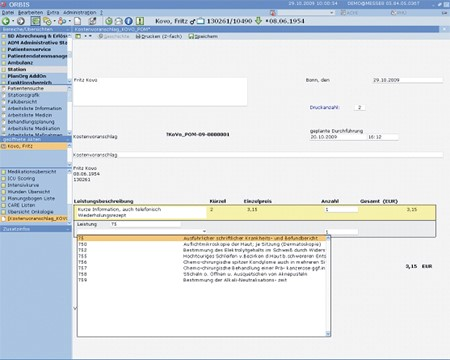
\includegraphics[width=0.6\textwidth]{orbis2}
		  \caption{Orbis Module for diagnosis and medical reports. Users can
		  select the diagnosis from a defined catalogue and write a free text to the
		  medical report which is stored as a PDF file in the Electronic Medical
		  Record.}
	\end{figure}
	\subsection{Orbis Database}
	The Orbis Database has grown over years. At the beginning it was a small
	database for a small application to store patient data. Because of the user
	requirements, the company AGFA has built additional features. \\
	On the one hand, they developed additional features and modules for the
	application and on the other they bought applications and companies, which had developed
	the applications and merged those with Orbis. Therefore, the database grew
	more and more and new schemes and tables were added. This development led to
	the main problem: a bad performance for users.
	\subsection{Actual Problems}
	The actual problem is that many database models were merged. Many of
	them are not stateoftheart. So there are really big database tables with
	many columns without primary keys. They don't have foreign keys to
	other tables. Sometimes it is not easy to make a join over different tables.\\
	Another problem is to get a general overview of the Orbis-database, because
	of the problems described above. This makes it necessary to get and define simple values, which are displayed in the application as well. Deep
	knowledge of the Orbis-database is necessary.
	\subsection{Reports for Orbis}
	It was a goal of the project to build reports for the Board of Directors with
	the Orbis database in IBM Cognos. 
	\subsubsection{Overview about the reports}
	A Cognos Cube was built with AGFA and a server job was developed
	to get current data from the Orbis Database to these Cognos Cube.
	The next step was to use the IBM Cognos Report Studio to develop reports for
	Web-Browser in HTML and for iPhone applications.
	\begin{figure}[!ht]
		  \centering
		      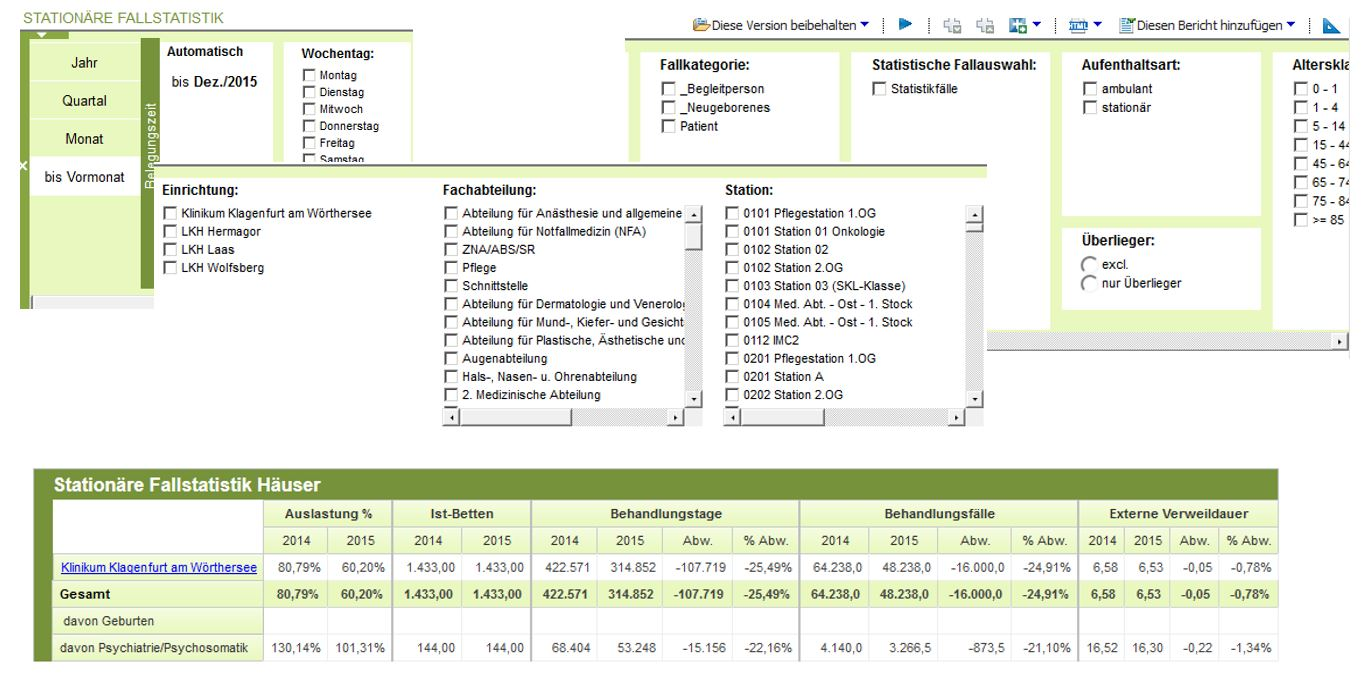
\includegraphics[width=1.0\textwidth]{reports_overview}
		  \caption{An overview of one of the reports. It is
		  possible to select the hospital, department and station and more.}
	\end{figure}
	\subsubsection{Result of the report}
	The results of the reports the boards of directors will get are displayed in
	tables, charts and diagrams. So it will be simple for them to present statistical key figures from the Hospital Information System and the
	billing and other statistics.
	\begin{figure}[!ht]
		  \centering
		      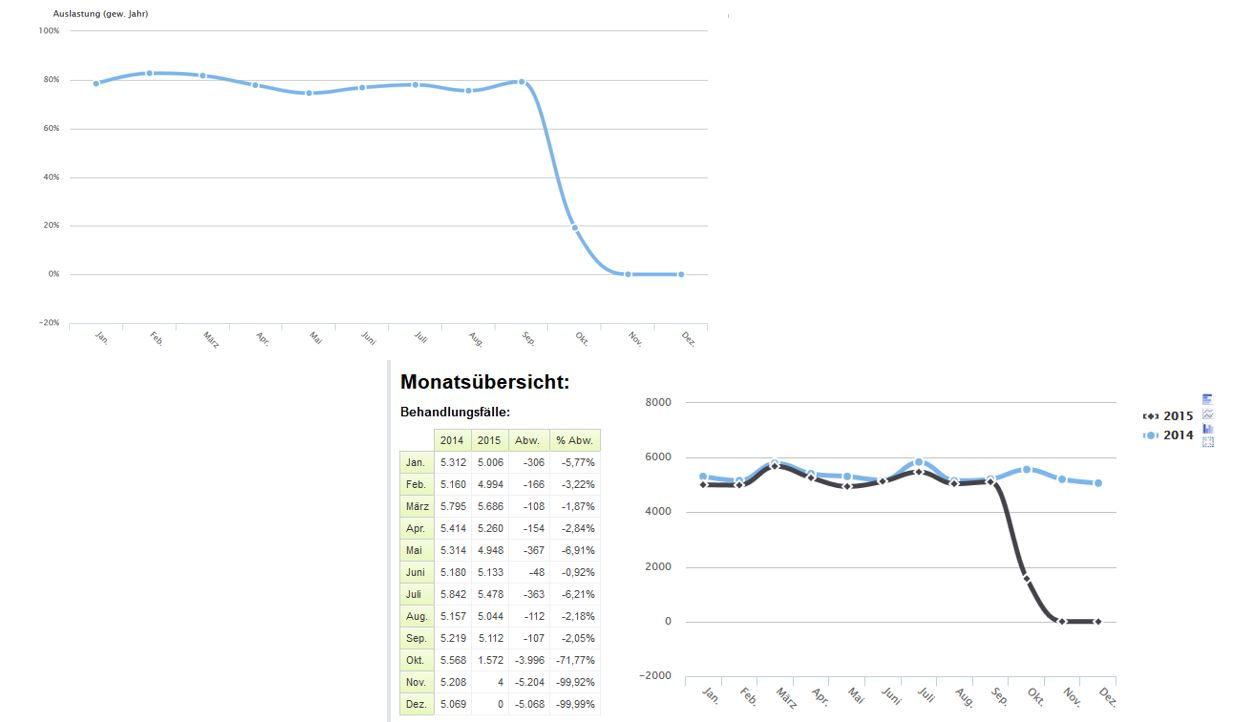
\includegraphics[width=1.0\textwidth]{reports_results}
		  \caption{An example of a report for the in-patient statistics of the
		  Klinikum Klagenfurt. The load factor of the Klinikum is shown. The curve decreases to zero on October.}
	\end{figure}

\end{document}
